\chapter{Actieve Systemen}
\begin{itemize}
	\item Klassieke regelbanken worden gebruikt voor expertsystemen, die toelaten om conclusies te trekken uit bepaalde gegevens.
	\item Er kan ook een systeem ontwikkeld worden waar het geheel
\end{itemize}
\section{Eenvoudige systemen}
\begin{itemize}
	\item Bij een eenvoudig systeem is het mogelijk een opsomming te maken van alle visies, acties en hun combinaties.
	\item Bij elke tijdsstap analyseert de actieve eenheid de visie en kiest op basis daarvan een actie. De buitenwereld reageert op deze actie en genereert een nieuwe visie.
	\alert Een visie geeft slechts gedeeltelijke beschrijving van de wereld. Een \textbf{\gls{ac:hmdm}}, wat een uitbreiding is op een \textbf{\gls{ac:hmm}}, tracht dit te modelleren en bestaat uit het volgende:
	\begin{itemize}
		\item Een eindige verzameling van \textbf{staten} $S = \{s_1, ..., s_n\}$. Er is een beginstaat $(s_1)$ en een eindstaat $(s_n)$.
		\item Een eindige verzameling $D = \{d_1, ..., d_l\}$ van \textbf{beslissingen}.
		\item Voor elke $d \in D$ een \textbf{transitiematrix} $T(d)$.
		\item Een \textbf{uitvoeralfabet} $A = \{a_1, ..., a_k\}$. Dit is het alfabet van visies.
		\item Een \textbf{beloningsfunctie} $b: A \rightarrow \mathcal{R}$. Een beloning kan negatief zijn.
		\item Een $n \times k$ \textbf{uitvoermatrix} $U$.
	\end{itemize}
	\item Een \textbf{run} is het hele proces van begintoestand en eindtoestand. 
	\item Een actieve eenheid moet een \textbf{strategie} $\tau$ hebben. Aan elke letter $a$ van het uitvoeralfabet is er dan een beslissing $\tau(a)$.
	\item \underline{Actieve eenheden zonder onzekerheid:} twee voorwaarden
	\begin{enumerate}
		\item \begin{itemize}		
			\item De staat komt overeen met de visie.
			\item Er is een één op één relatie tussen A en S, waarbij $k = n$ en $U$ een diagonaalmatrix waarbij alle diagonaalelementen 1 zijn.
			\item Noteer $\tau(s) = d$ als een strategie $\tau$ die in staat $s$ beslissing $d$ neemt.
			\item Dit zorgt ervoor dat dat de H uit \gls{ac:hmdm} mag wegvallen.
			\end{itemize}
		\item \begin{itemize}
			\item De overgang naar de volgende staat is helemaal gedetermineerd door de beslissing. 
			\item Elke $T(d)_{ij}$ is ofwel 1 ofwel 0. 
			\item De transitie kan uitgedrukt worden als $T(d, s) = s'$ als $d$ leidt tot een overgang naar staat $s'$.
			\item We krijgen een deterministisch systeem waarbij een staat $s$ in één tijdsstap overgaat in de staat $T(\tau(s), s)$.
	\end{itemize}
	\end{enumerate}
	\item \underline{Voorbeeld: figuur \ref{fig:doolhof_exploratie}} 
	\begin{figure}[ht]
		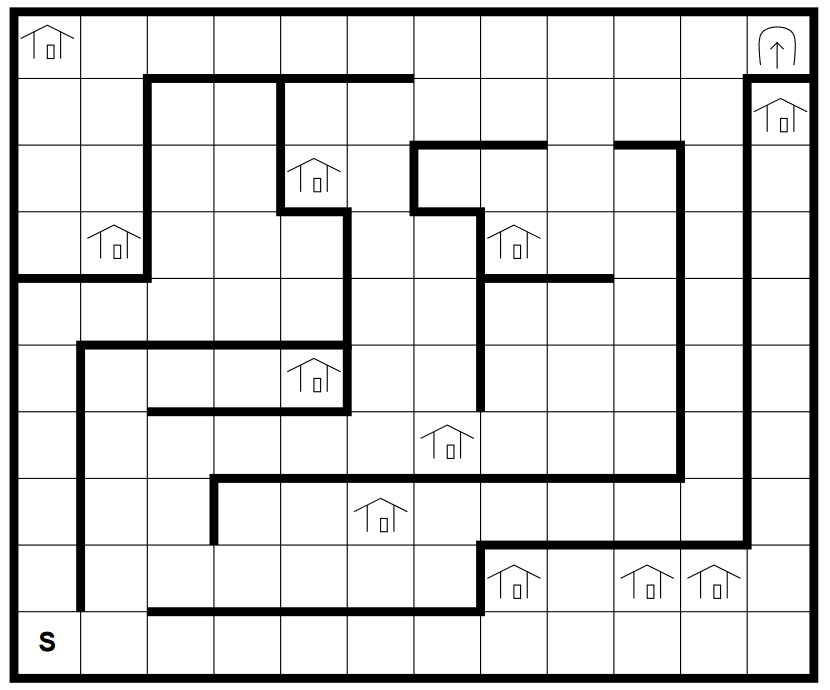
\includegraphics[width=\linewidth]{doolhof_exploratie}
		\caption{Een eenvoudige leerwereld.}
		\label{fig:doolhof_exploratie}
	\end{figure}
	\begin{itemize}
		\item Een doolhof met startpositie $s$.
		\item Op elke plaats kan de eenheid beslissen één vakje verder te gaan in horizontale of verticale richting. De eenheid kan niet door dikke lijnen heen.
		\item Het verplaatsen van een vakje naar een volgend vakje kost 1 dag.
		\item De eenheid kan maar voor 10 dagen verplaatsingen doen.
		\item Een hut kan onbeperkt het aantal dagen terug opvullen tot 10.
		\alert We gaan ervan uit dat er geen lussen zijn in het optimale pad. De eenheid zal dus niet telkens twee hutten oneindig lang blijven bezoeken.
		\item De eenheid moet nu met zoveel mogelijk dagen de uitgang (rechtsboven) weten te bereiken. 
		\item Om een MDM te maken wordt voor elk vakje 11 staten bijgehouden. Bij elke staat wordt de coördinaten van het vakje aangevuld met het aantal dagen van de eenheid bijgehouden.
		\item De beginstaat is dan $((0, 0), 10)$.
		\item Er kan aan elke staat een waarde gegeven worden:
		\begin{itemize}
			\item Voor de eindstaten waar de eenheid sterft is de waarde -10.
			\item Voor de eindstaten aan de uitgang, $((11, 9), i)$ is de waarde $i + 1$.
			\item Voor de andere vakjes is er een verband tussen de waardering voor de staat door eenheid en de gevolgde strategie.
		\end{itemize}
		\item In het algemeen geval wordt de formule gegeven:
		{\color{OliveGreen}	$$\omega_\pi(s) = b(s) + \omega_\pi(T(\pi(s), s))$$}
		\begin{itemize}
			\item De strategie $\pi$ beïnvloedt de waarde $\omega_\pi(s)$ als $\pi$ toegepast wordt op een staat $s$.
		\end{itemize}
		\item Aangezien er geen onzekerheid is kan een optimale strategie $\tau_{opt}$ gevonden worden zodat $\omega_{\tau_{opt}}(s) \geq \omega_\tau(s)$. De beslissing $\tau_{opt}(s)$ leidt dan tot een staat $s'$ die voldoet aan
		{\color{OliveGreen}		
		$$\omega_{\tau_{opt}}(s) = b(s) + \max_{\substack{d \in D}} \omega_{\tau_{opt}}(T(d,s))$$
		}
	\item Het kan zijn dat er meerdere optimale strategieën bestaan. De formule kan dan herschreven worden door het maximum van alle strategieën te pakken, zodat de keuze van strategie niet meer uitmaakt:
		{\color{OliveGreen}		
		$$w^*(s) = b(s) + \max_{\substack{\tau}}\omega_\tau(T(d, s))$$
	}
	Voor elke optimale strategie geldt dat $\omega_{\tau_{opt}}(s) = \omega^*(s) $
	\end{itemize}
\end{itemize}

\subsection{Exploratie zonder onzekerheid}
\begin{itemize}
	\item Een \textbf{exploratiestrategie} laat de eenheid leren door te zien wat er gebeurt.
	\item Een klassieke strategie neemt elke keer dezelfde beslissing voor elke staat.
	\item Een exploratiestrategie $\xi$ kent aan elke combinatie $(s, d)$ een probabiliteit $\xi(s, d)$ toe. Hierbij geldt:
	$$\sum_D \xi(s, d) = 1$$
	\item Als de eenheid in staat $s$ terechtkomt, wordt beslissing $d$ gekozen op basis van de probabiliteit.
	\item De totale opbrengst $W$ kan voor een specifieke run bepaald worden. Voor alle staten die de eenheid gepasseerd is, kan de benaderde schatting $\omega(s)$ van $\omega^*(s)$ vervangen worden door
	$$\max\{W, w(s)\}$$
\end{itemize}

\subsection{Exploratie met onzekerheid}
\begin{itemize}
	\item Hierbij is er geen één op één relatie tussen staat en visie. De overgang naar een nieuwe staat is slechts probabilistisch afhankelijk van de genomen beslissing.
	\item Gegeven een staat $s_i$ en een beslissing $d$, dan is de waarschijnlijkheid om over te gaan naar $s_j$ gelijk aan $T(d)_{ij}$. 
	\begin{itemize}
		\alert Dit heeft als gevolg dat de winst van een strategie $\pi$ niet exact kan voorspeld worden als we uit een staat $s$ vertrekken.
		\item Er kan wel een \textbf{verwachtingswaarde} berekend worden:
		{\color{OliveGreen}
		$$\omega_\pi(s_i) = b(s_i) + \sum_j T(\pi(s_i))_{ij}\omega_\pi(s_j)$$
		}
	\end{itemize}
	\item Een lerende eenheid kent het systeem echter niet. Het moet niet alleen een schatting maken van de waarde van alle staten, maar ook van de overgangswaarschijnlijkheden $T(d)_{ij}$. Stel $A_{ij}$ het totaal aantal keer dat de eenheid in staat $s_j$ is geraakt vanuit staat $s_i$ door $d$ te gebruiken, dan wordt volgende schatting gebruikt:
	$$T(d)_{ij} \approx \frac{A_{ij}}{\sum_{k=1}^{n}A_{ik}}$$
\end{itemize}

\section{Complexe systemen}
\begin{itemize}
	\item Bij eenvoudige systemen is er informatie beschikbaar over elke staat. Bij systemen met onzekerheid moet zelf voor elke combinatie $(s, d)$ de overgangswaarschijnlijkheid naar elke staat bijgehouden worden.
	\alert Niet haalbaar voor een groot aantal staten.
	\item Invoering van \textbf{actieve regelbanken}, deze bevat regels van de vorm
			\begin{equation*}
				\begin{split}
				& \hbox{\textbf{als} premisse} \\
				& \hbox{\textbf{dan} voer actie uit} 
				\end{split}
			\end{equation*}
	\good Eenvoudiger dan klassieke regelbanken: een actie kan geen deel uitmaken van de premisse van een andere regel.
	\item Om de actieve regelbank zo klein mogelijk te houden worden regels zo algemeen mogelijk genomen. In het geval van conflicten zoals
				\begin{equation*}
					\begin{split}
					& \hbox{\textbf{als} } a > 3 \hbox{ en } a \leq 5 \\
					& \hbox{\textbf{dan} voer actie 1 uit} 
					 \\[3ex]
					& \hbox{\textbf{als} } b == 2 \\
					& \hbox{\textbf{dan} voer actie 2 uit} \\
					\end{split}
				\end{equation*}
	wordt meestal de regel gekozen die het minst algemeen is. In sommige gevallen wordt er ook randomisatie gebruikt om variatie te hebben tussen acties.
	\item Actieve regelbanken worden gebruikt bij genetische algoritmen.
\end{itemize}

\section{Genetische algoritmen}
\begin{figure}
	
	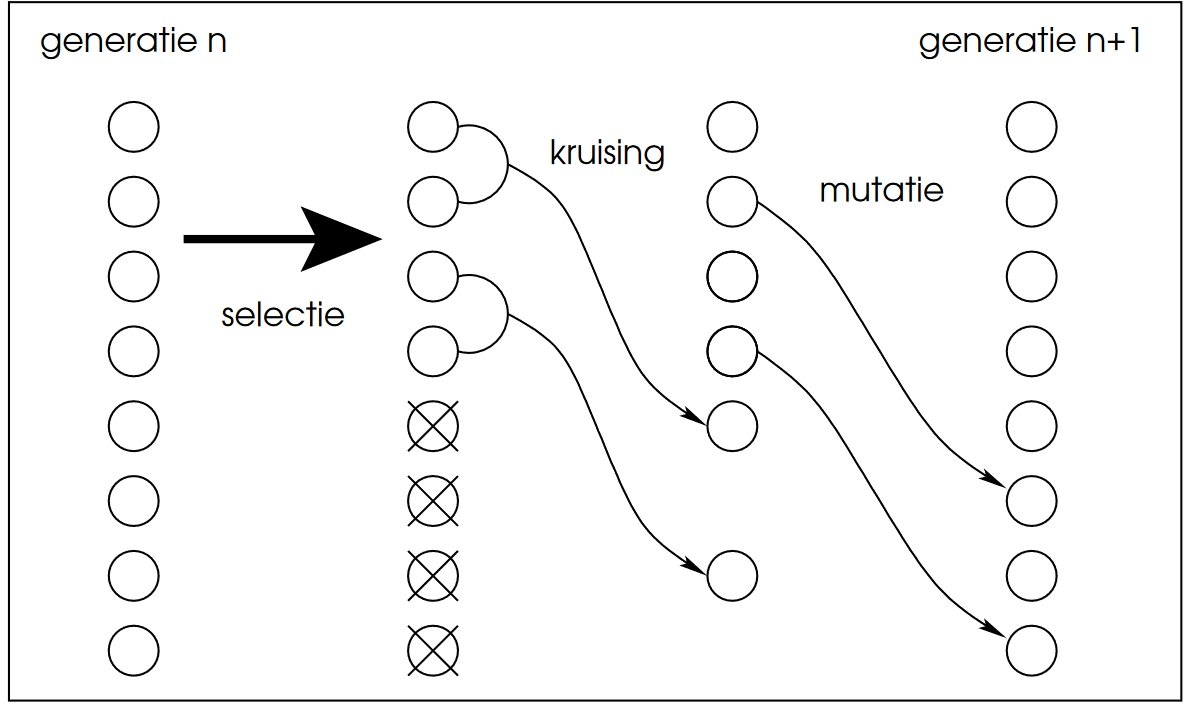
\includegraphics[width=\textwidth]{genetisch_algoritme}
\end{figure}
\begin{itemize}
	\item Start vanuit een grote groep van strategieën, de \textbf{populatie}.
	\item Wijzig nu de populatie door strategieën te verwijderen, toe te voegen of aan te passen zodat uiteindelijk een strategie gevonden is die efficiënt is.
	\item We maken gebruik van \textbf{generaties}. Elke generatie bestaat uit een populatie die even groot is. De volgende generatie wordt bekomen in twee stappen:
	\begin{enumerate}
		\item De populatie wordt uitgedund zodat enkel de beste strategieën overblijven.
		\begin{itemize}
			\item Er moet een \textbf{geschiktheidsfunctie} gedefinieerd worden.
			
		\end{itemize}
		\item Gebaseerd op de overblijvende strategieën wordt de populatie terug aangevuld. Hier kan er kruising of mutatie toegepast worden. 
		\begin{itemize}
			\item Een \textbf{kruising} neemt twee exemplaren uit de populatie en vermengt deze, zodat de nakomeling eigenschappen heeft van de ouders.
			\item Een \textbf{mutatie} voert een kleine wijziging door aan een strategie uit de populatie.
		\end{itemize}
	\end{enumerate}
	\item \underline{Voorbeeld: uurroosterprobleem}
	\begin{itemize}
		\item Er zijn een aantal studentengroepen die elk een aantal cursussen volgen die gegeven worden door bepaalde docenten. Verder zijn er klaslokalen.
		\item Er moet een uurrooster opgemaakt worden dat aan een aantal eisen voldoet. Er zijn twee soorten eisen:
		\begin{enumerate}
			\item \textbf{Harde eisen}: \begin{itemize}
				\item Elke cursus moet gegeven worden.
				\item Een docent kan maar één cursus geven op een moment.
				\item Een studentengroep kan maar les volgen op één moment.
				\item Elke les moet doorgaan in een lokaal dat geschikt is voor de les.
				\item Er kunnen geen twee lessen tegelijk doorgaan in hetzelfde lokaal.
			\end{itemize}
			\item \textbf{Zachte eisen}:
			\begin{itemize}
				\item Er moeten zo weinig mogelijk springuren zijn.
				\item De lokaalwissels moeten beperkt blijven.
				\item enz...
			\end{itemize}
		\end{enumerate}
		\item De beginpopulatie kan nooit aan alle voorwaarden voldoen. Daarom worden onmogelijke uurroosters toegelaten, maar deze krijgen een slechte geschiktheid. 
		\begin{enumerate}
			\item Voor elke harde eis die niet voldaan is worden duizend strafpunten afgetrokken.
			\item Voor elke zachte eis die niet voldaan is wordt één punt afgetrokken.
		\end{enumerate}

	\end{itemize}
\end{itemize}

\section{Optimalisatie van één strategie}
\section{Combinaties}

